
\section{Results}
In this section, we present results of the performance for pattern matching of the two graph databases: Neo4j and OrientDB. In ~\ref{setup}, we provide details of the machine used for the experiments and in ~\ref{result}, we presents the results and discuss the optimization we did to run the pattern matching queries terminate faster.

\subsection{Experimental Setup}
\label{setup}

The machine we used for our experiment was large memory machine (256 GB): 2 socket Intel(R) Xeon(R) CPU E5-2650 @ 2.00GHz processors (32 cores). This machine was large enough to load IMDB graph ~\cite{IMDb96:online} in the memory.

\subsection{Results}
\label{result}
We obtained the results by running one pattern matching query on one database at a time to make sure that the query performance is not impacted due to other queries on the databases.

We started with pattern matching query P1 on the Neo4j database and to our surprise, it took around 9 hours for the query to terminate. Hence, we tried to optimize the query by running the query in the multiple threads at a time. As there were 32 cores on the machine and total of around 3.6 million person vertices (actors, actresses, and directors) to run the pattern matching query. Hence, we first use 20 threads for first 2 million and then 17 threads for remining using pool of threads. With each thread processing 100,000 vertices, total time for P1 reduced to around 30 minutes for Neo4j. We did the same optimization for two other queries and for both graph databases.

We ran the the pattern matching queries for both databases and the results are show in the figure ~\ref{fig:comparsion}

\begin{figure}[h!]
	\centering
	\resizebox{0.5\linewidth}{!}{
		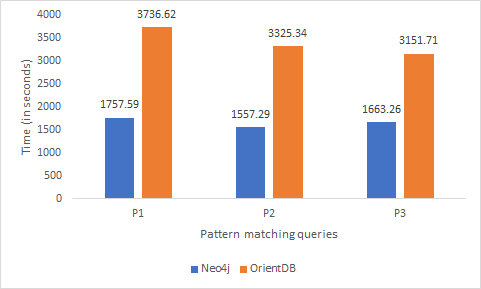
\includegraphics[width=0.8\linewidth]{Images/comparison.png}
	}
	\caption{Graph databases: Performance comparison}
	\label{fig:comparsion}
	\centering
\end{figure}

We can see from the figure ~\ref{fig:comparsion} that the Neo4j's performance is better than OrientDB by at least 2 times.

\section{Conclusions}
From the experimental results, it is clear that the Neo4j performs better than OrientDB. From our experience, we can say that not all the Gremlin queries are supported in the OrientDB. We also found that there were various versions mismatch issue between the database, Gremlin, and libraries for which we had to do lot of trial and error to make the experiment work.

\section{Future Work}
OrientDB and Neo4j both claim to be a native graph database. OrientDB supports multi-models such as key-value store, a document store, and graph database. as such it's a graph database with nodes as document. Neo4j only allows graph to be stored as property graph. From the results we got, it definitely seems that Neo4j is more optimized when compared to orientDB. Study of optimizations that contributed for Neo4j to perform better will be a future work for this project.   

\begin{comment}
\begin{table}[h!]
\resizebox{0.3\textwidth}{!}{%
\begin{tabular}{ |c|c|c| } 
\hline
& Neo4j & OrientDB \\ 
\hline
P1 & 1757.59 & 3736.62 \\ 
\hline
P2 & 1557.29 & 3325.34 \\ 
\hline
P3 & 1663.26 & 3151.71 \\
\hline
\end{tabular}
}%resizebox
\caption{Pattern matching performance comparison}
\label{table}
\end{table}
\end{comment}